\documentclass[11pt, a4paper]{article}
\usepackage{amsmath, amssymb, booktabs, geometry, hyperref, xcolor, listings}
\usepackage{tikz}
\usetikzlibrary{shapes.geometric, arrows.meta, positioning, calc}
\geometry{margin=2.5cm}
\hypersetup{colorlinks=true, linkcolor=blue, urlcolor=blue}
\lstset{basicstyle=\ttfamily\small, backgroundcolor=\color{gray!10}, frame=single}

\title{\textbf{Portfolio Value-at-Risk Engine}\\[4pt]
\large Model Overview and Framework Documentation}
\author{Risk Modelling --- Trade Republic}
\date{April 2026}

\begin{document}
\maketitle
\tableofcontents
\newpage

%-----------------------------------------------------------------------
\section{Introduction}

This document provides an overview of the \texttt{portfolio\_vaR} engine
implemented in \texttt{risk\_analytics.risk\_engines} (file:
\texttt{risk\_pylibrary/risk\_analytics/risk\_engines.py}).

The engine computes one-step-ahead (or multi-day) portfolio
\textbf{Value-at-Risk (VaR)} and \textbf{Conditional Value-at-Risk (CVaR,
Expected Shortfall)} for a weighted asset portfolio. Five distinct risk
methodologies are available, selected via the \texttt{engine} parameter.

%-----------------------------------------------------------------------
\section{Code Flowchart}

Figure~\ref{fig:flowchart} shows the full execution path of
\texttt{portfolio\_vaR()}, from input validation through engine dispatch
to the final output DataFrame.

\begin{figure}[htbp]
\centering
\resizebox{\textwidth}{!}{%
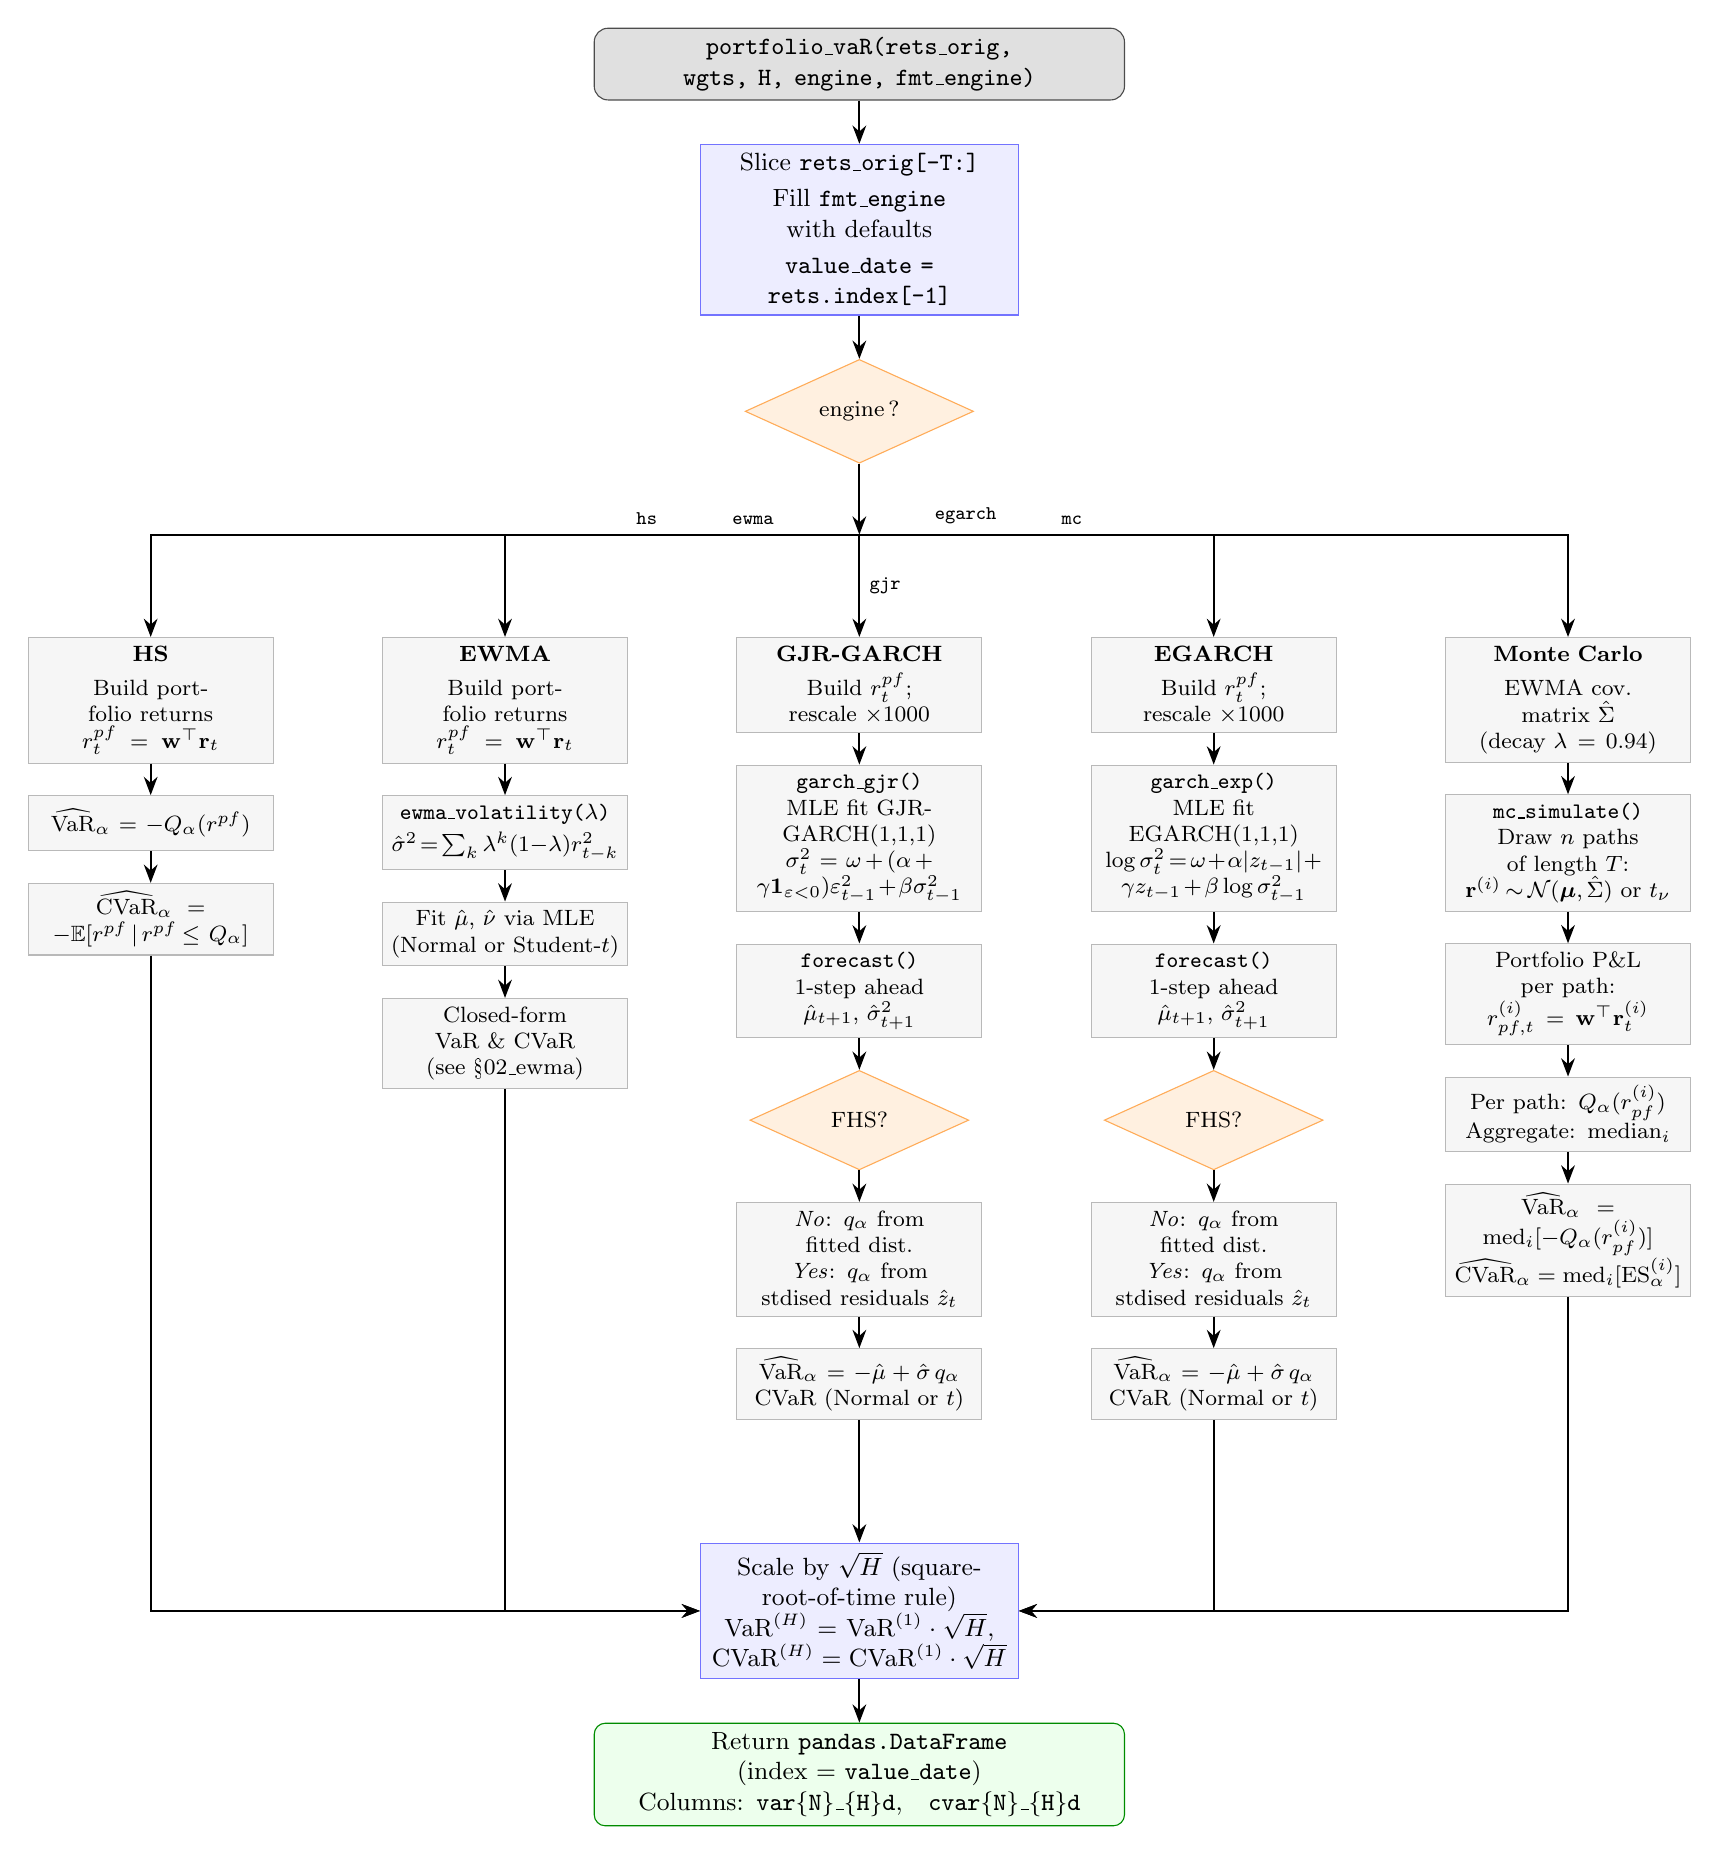
\begin{tikzpicture}[
  node distance = 0.45cm,
  %-- styles --
  startend/.style = {
    rectangle, rounded corners=5pt,
    draw=black!70, fill=black!12,
    text width=6.5cm, align=center,
    font=\small\bfseries, minimum height=0.9cm
  },
  proc/.style = {
    rectangle, draw=blue!55, fill=blue!7,
    text width=3.8cm, align=center,
    font=\small, minimum height=0.75cm
  },
  engbox/.style = {
    rectangle, draw=gray!55, fill=gray!7,
    text width=2.9cm, align=center,
    font=\footnotesize, minimum height=0.7cm,
    inner sep=3pt
  },
  deci/.style = {
    diamond, aspect=2.2,
    draw=orange!65, fill=orange!12,
    text width=1.6cm, align=center,
    font=\footnotesize
  },
  outbox/.style = {
    rectangle, rounded corners=4pt,
    draw=green!55!black, fill=green!7,
    text width=6.5cm, align=center,
    font=\small, minimum height=0.9cm
  },
  arr/.style  = {-Stealth, thick},
  darr/.style = {-Stealth, thick, gray!60},
]

%% ─────────────────────────────────────────────────────────────────────
%% TOP: function call
%% ─────────────────────────────────────────────────────────────────────
\node[startend] (call) {
  \texttt{portfolio\_vaR(rets\_orig, wgts, H, engine, fmt\_engine)}
};

\node[proc, below=0.55cm of call] (prep) {
  Slice \texttt{rets\_orig[-T:]}\\[2pt]
  Fill \texttt{fmt\_engine} with defaults\\[2pt]
  \texttt{value\_date = rets.index[-1]}
};

\node[deci, below=0.55cm of prep] (dispatch) {engine\,?};

%% ─────────────────────────────────────────────────────────────────────
%% FIVE BRANCHES  (centred at x = -9, -4.5, 0, +4.5, +9)
%% ─────────────────────────────────────────────────────────────────────

%%── HS ──────────────────────────────────────────────────────────────
\node[engbox, below=2.2cm of dispatch, xshift=-9cm] (hs1) {
  \textbf{HS}\\[3pt]
  Build portfolio returns\\
  $r_t^{pf} = \mathbf{w}^\top \mathbf{r}_t$
};
\node[engbox, below=0.4cm of hs1] (hs2) {
  $\widehat{\text{VaR}}_\alpha = -Q_\alpha(r^{pf})$
};
\node[engbox, below=0.4cm of hs2] (hs3) {
  $\widehat{\text{CVaR}}_\alpha =$\\
  $-\mathbb{E}[r^{pf}\,|\,r^{pf}\!\leq Q_\alpha]$
};

%%── EWMA ─────────────────────────────────────────────────────────────
\node[engbox, below=2.2cm of dispatch, xshift=-4.5cm] (ew1) {
  \textbf{EWMA}\\[3pt]
  Build portfolio returns\\
  $r_t^{pf} = \mathbf{w}^\top \mathbf{r}_t$
};
\node[engbox, below=0.4cm of ew1] (ew2) {
  \texttt{ewma\_volatility($\lambda$)}\\[2pt]
  $\hat\sigma^2 \!=\! \sum_{k}\lambda^k(1{-}\lambda)r_{t-k}^2$
};
\node[engbox, below=0.4cm of ew2] (ew3) {
  Fit $\hat\mu$, $\hat\nu$ via MLE\\
  (Normal or Student-$t$)
};
\node[engbox, below=0.4cm of ew3] (ew4) {
  Closed-form VaR \& CVaR\\
  (see \S02\_ewma)
};

%%── GJR-GARCH ────────────────────────────────────────────────────────
\node[engbox, below=2.2cm of dispatch, xshift=0cm] (gjr1) {
  \textbf{GJR-GARCH}\\[3pt]
  Build $r_t^{pf}$; rescale $\times1000$
};
\node[engbox, below=0.4cm of gjr1] (gjr2) {
  \texttt{garch\_gjr()}\\
  MLE fit GJR-GARCH(1,1,1)\\
  $\sigma_t^2\!=\!\omega\!+\!(\alpha\!+\!\gamma\mathbf{1}_{\varepsilon<0})\varepsilon_{t-1}^2\!+\!\beta\sigma_{t-1}^2$
};
\node[engbox, below=0.4cm of gjr2] (gjr3) {
  \texttt{forecast()} 1-step ahead\\
  $\hat\mu_{t+1}$,\ $\hat\sigma_{t+1}^2$
};
\node[deci, below=0.4cm of gjr3] (gjr4) {FHS?};
\node[engbox, below=0.4cm of gjr4] (gjr5) {
  \textit{No}: $q_\alpha$ from fitted dist.\\
  \textit{Yes}: $q_\alpha$ from\\stdised residuals $\hat z_t$
};
\node[engbox, below=0.4cm of gjr5] (gjr6) {
  $\widehat{\text{VaR}}_\alpha = -\hat\mu + \hat\sigma\,q_\alpha$\\
  CVaR (Normal or $t$)
};

%%── EGARCH ───────────────────────────────────────────────────────────
\node[engbox, below=2.2cm of dispatch, xshift=+4.5cm] (eg1) {
  \textbf{EGARCH}\\[3pt]
  Build $r_t^{pf}$; rescale $\times1000$
};
\node[engbox, below=0.4cm of eg1] (eg2) {
  \texttt{garch\_exp()}\\
  MLE fit EGARCH(1,1,1)\\
  $\log\sigma_t^2\!=\!\omega\!+\!\alpha|z_{t-1}|\!+\!\gamma z_{t-1}\!+\!\beta\log\sigma_{t-1}^2$
};
\node[engbox, below=0.4cm of eg2] (eg3) {
  \texttt{forecast()} 1-step ahead\\
  $\hat\mu_{t+1}$,\ $\hat\sigma_{t+1}^2$
};
\node[deci, below=0.4cm of eg3] (eg4) {FHS?};
\node[engbox, below=0.4cm of eg4] (eg5) {
  \textit{No}: $q_\alpha$ from fitted dist.\\
  \textit{Yes}: $q_\alpha$ from\\stdised residuals $\hat z_t$
};
\node[engbox, below=0.4cm of eg5] (eg6) {
  $\widehat{\text{VaR}}_\alpha = -\hat\mu + \hat\sigma\,q_\alpha$\\
  CVaR (Normal or $t$)
};

%%── MONTE CARLO ──────────────────────────────────────────────────────
\node[engbox, below=2.2cm of dispatch, xshift=+9cm] (mc1) {
  \textbf{Monte Carlo}\\[3pt]
  EWMA cov.\ matrix $\hat\Sigma$\\
  (decay $\lambda = 0.94$)
};
\node[engbox, below=0.4cm of mc1] (mc2) {
  \texttt{mc\_simulate()}\\
  Draw $n$ paths of length $T$:\\
  $\mathbf{r}^{(i)}\!\sim\!\mathcal{N}(\boldsymbol\mu,\hat\Sigma)$ or $t_\nu$
};
\node[engbox, below=0.4cm of mc2] (mc3) {
  Portfolio P\&L per path:\\
  $r_{pf,t}^{(i)} = \mathbf{w}^\top\mathbf{r}_t^{(i)}$
};
\node[engbox, below=0.4cm of mc3] (mc4) {
  Per path: $Q_\alpha(r_{pf}^{(i)})$\\
  Aggregate: $\text{median}_i$
};
\node[engbox, below=0.4cm of mc4] (mc5) {
  $\widehat{\text{VaR}}_\alpha = \text{med}_i[-Q_\alpha(r_{pf}^{(i)})]$\\
  $\widehat{\text{CVaR}}_\alpha = \text{med}_i[\text{ES}_\alpha^{(i)}]$
};

%% ─────────────────────────────────────────────────────────────────────
%% FOOTER: scaling + output
%% ─────────────────────────────────────────────────────────────────────
\node[proc, below=13.7cm of dispatch] (scale) {
  Scale by $\sqrt{H}$ (square-root-of-time rule)\\
  $\text{VaR}^{(H)} = \text{VaR}^{(1)}\cdot\sqrt{H}$,\quad
  $\text{CVaR}^{(H)} = \text{CVaR}^{(1)}\cdot\sqrt{H}$
};

\node[outbox, below=0.55cm of scale] (output) {
  Return \texttt{pandas.DataFrame}\ (index = \texttt{value\_date})\\
  Columns: \texttt{var\{N\}\_\{H\}d},\quad \texttt{cvar\{N\}\_\{H\}d}
};

%% ─────────────────────────────────────────────────────────────────────
%% ARROWS: top
%% ─────────────────────────────────────────────────────────────────────
\draw[arr] (call) -- (prep);
\draw[arr] (prep) -- (dispatch);

%% ─────────────────────────────────────────────────────────────────────
%% ARROWS: dispatch → branch tops  (go down 1cm then fan out)
%% ─────────────────────────────────────────────────────────────────────
\coordinate (jct) at ($(dispatch.south) + (0,-0.9)$);
\draw[arr] (dispatch.south) -- (jct);

\draw[arr] (jct) -| node[above, pos=0.15, font=\scriptsize] {\texttt{hs}}     (hs1.north);
\draw[arr] (jct) -| node[above, pos=0.15, font=\scriptsize] {\texttt{ewma}}   (ew1.north);
\draw[arr] (jct) -- node[right,            font=\scriptsize] {\texttt{gjr}}    (gjr1.north);
\draw[arr] (jct) -| node[above, pos=0.15, font=\scriptsize] {\texttt{egarch}} (eg1.north);
\draw[arr] (jct) -| node[above, pos=0.15, font=\scriptsize] {\texttt{mc}}     (mc1.north);

%% ─────────────────────────────────────────────────────────────────────
%% ARROWS: internal branch flows
%% ─────────────────────────────────────────────────────────────────────

% HS
\draw[arr] (hs1) -- (hs2);
\draw[arr] (hs2) -- (hs3);

% EWMA
\draw[arr] (ew1) -- (ew2);
\draw[arr] (ew2) -- (ew3);
\draw[arr] (ew3) -- (ew4);

% GJR
\draw[arr] (gjr1) -- (gjr2);
\draw[arr] (gjr2) -- (gjr3);
\draw[arr] (gjr3) -- (gjr4);
\draw[arr] (gjr4) -- (gjr5);
\draw[arr] (gjr5) -- (gjr6);

% EGARCH
\draw[arr] (eg1) -- (eg2);
\draw[arr] (eg2) -- (eg3);
\draw[arr] (eg3) -- (eg4);
\draw[arr] (eg4) -- (eg5);
\draw[arr] (eg5) -- (eg6);

% MC
\draw[arr] (mc1) -- (mc2);
\draw[arr] (mc2) -- (mc3);
\draw[arr] (mc3) -- (mc4);
\draw[arr] (mc4) -- (mc5);

%% ─────────────────────────────────────────────────────────────────────
%% ARROWS: branch bottoms → scale node
%% ─────────────────────────────────────────────────────────────────────
\draw[arr] (hs3.south)  -- ++(0,-0.4) |- (scale.west);
\draw[arr] (ew4.south)  -- ++(0,-0.4) |- (scale.west);
\draw[arr] (gjr6.south) --               (scale.north);
\draw[arr] (eg6.south)  -- ++(0,-0.4) |- (scale.east);
\draw[arr] (mc5.south)  -- ++(0,-0.4) |- (scale.east);

\draw[arr] (scale) -- (output);

\end{tikzpicture}
}% end resizebox
\caption{Execution flowchart of \texttt{portfolio\_vaR()} in
  \texttt{risk\_analytics/risk\_engines.py}.
  The central GJR-GARCH and EGARCH branches share the same
  VaR/CVaR calculation logic via \texttt{calculate\_vaR\_garch()}.}
\label{fig:flowchart}
\end{figure}

%-----------------------------------------------------------------------
\section{Notation}

\begin{tabular}{ll}
\toprule
Symbol & Description \\
\midrule
$r_{i,t}$ & Daily return of asset $i$ at time $t$ \\
$w_i$ & Portfolio weight of asset $i$, $\sum_i w_i = 1$ \\
$r_t^{pf}$ & Portfolio return: $r_t^{pf} = \sum_i w_i r_{i,t}$ \\
$T$ & Lookback window (default: 250 trading days) \\
$H$ & Holding period (default: 1 day) \\
$\alpha$ & Loss probability level, e.g.\ $\alpha \in \{0.05, 0.01, 0.001\}$ \\
$\lambda$ & EWMA decay factor (default: 0.94) \\
$\nu$ & Student-$t$ degrees of freedom \\
\bottomrule
\end{tabular}

%-----------------------------------------------------------------------
\section{Available Engines}

\begin{tabular}{lll}
\toprule
\texttt{engine} key & Model & Distribution options \\
\midrule
\texttt{hs}    & Historical Simulation          & non-parametric \\
\texttt{ewma}  & EWMA Volatility (parametric)   & Normal, Student-$t$ \\
\texttt{gjr}   & GJR-GARCH(1,1,1)              & Normal, Student-$t$ \\
\texttt{egarch}& EGARCH(1,1,1)                  & Normal, Student-$t$ \\
\texttt{mc}    & Multivariate Monte Carlo        & Normal, Student-$t$ \\
\bottomrule
\end{tabular}

%-----------------------------------------------------------------------
\section{Common Output Format}

All engines return a \texttt{pandas.DataFrame} indexed by the value date
with columns named:
\begin{align*}
&\texttt{var}\underbrace{N}_{1000(1-\alpha)}\texttt{\_}\underbrace{H}_{}\texttt{d}
&&\text{(VaR at confidence level $1-\alpha$, $H$-day horizon)} \\
&\texttt{cvar}\underbrace{N}_{1000(1-\alpha)}\texttt{\_}\underbrace{H}_{}\texttt{d}
&&\text{(CVaR at confidence level $1-\alpha$, $H$-day horizon)}
\end{align*}
Examples with default quantiles $\alpha \in \{0.05, 0.01, 0.001\}$ and $H=1$:
\begin{itemize}
  \item \texttt{var950\_1d} --- 95\% 1-day VaR
  \item \texttt{var990\_1d} --- 99\% 1-day VaR
  \item \texttt{var999\_1d} --- 99.9\% 1-day VaR
  \item \texttt{cvar950\_1d} --- 95\% 1-day CVaR (Expected Shortfall)
\end{itemize}

%-----------------------------------------------------------------------
\section{Holding-Period Scaling}

All engines scale 1-day estimates to a $H$-day horizon using the
square-root-of-time rule:
\begin{equation}
\text{VaR}_\alpha^{(H)} = \text{VaR}_\alpha^{(1)} \cdot \sqrt{H}
\qquad
\text{CVaR}_\alpha^{(H)} = \text{CVaR}_\alpha^{(1)} \cdot \sqrt{H}
\label{eq:sqrt_rule}
\end{equation}
This assumes i.i.d.\ daily returns and is an approximation for correlated
(GARCH-type) processes.

%-----------------------------------------------------------------------
\section{Model Cross-Reference}

\begin{tabular}{lcccc}
\toprule
Engine & Parametric tail & Volatility clustering & Multivariate & Non-parametric tail \\
\midrule
HS     & --  & --  & -- & \checkmark \\
EWMA   & \checkmark & -- & -- & -- \\
GJR    & \checkmark & \checkmark & -- & optional (FHS) \\
EGARCH & \checkmark & \checkmark & -- & optional (FHS) \\
MC     & \checkmark & -- & \checkmark & -- \\
\bottomrule
\end{tabular}

%-----------------------------------------------------------------------
\section{Detailed Model Descriptions}

Each engine is documented in a dedicated file within this directory:
\begin{itemize}
  \item \texttt{model\_desc/hs/01\_historical\_simulation.tex}
  \item \texttt{model\_desc/ewma/02\_ewma.tex}
  \item \texttt{model\_desc/gjr\_garch/03\_gjr\_garch.tex}
  \item \texttt{model\_desc/egarch/04\_egarch.tex}
  \item \texttt{model\_desc/mc/05\_monte\_carlo.tex}
\end{itemize}

\end{document}
